\documentclass[journal,12pt,twocolumn]{IEEEtran}
\usepackage[none]{hyphenat}
\usepackage{graphicx}
\usepackage{listings}
\usepackage[english]{babel}
\usepackage{graphicx}
\usepackage{caption} 
\usepackage{amsmath}
\usepackage{hyperref}
\usepackage{booktabs}
\usepackage{array}
\usepackage{stix}


\title{\textbf{\\circle Assignment}}
\author{kanekal kousar}
\date{September 2022}

\providecommand{\norm}[1]{\left\lVert#1\right\rVert}
\providecommand{\abs}[1]{\left\vert#1\right\vert}
\let\vec\mathbf
\newcommand{\myvec}[1]{\ensuremath{\begin{pmatrix}#1\end{pmatrix}}}
\newcommand{\mydet}[1]{\ensuremath{\begin{vmatrix}#1\end{vmatrix}}}
\providecommand{\brak}[1]{\ensuremath{\left(#1\right)}}


\begin{document}
\maketitle


\section{Question}
\textbf{\textit{Q(6), C , Section-A, Chapter-8:}If a circle passes through the point (a,b)and cuts the circle {$x^2+y^2=k^2$} orthogonally, then the equation of the locus of its center is.}

\section{Solution}
\raggedright 

\begin{figure}[h!]
\centering
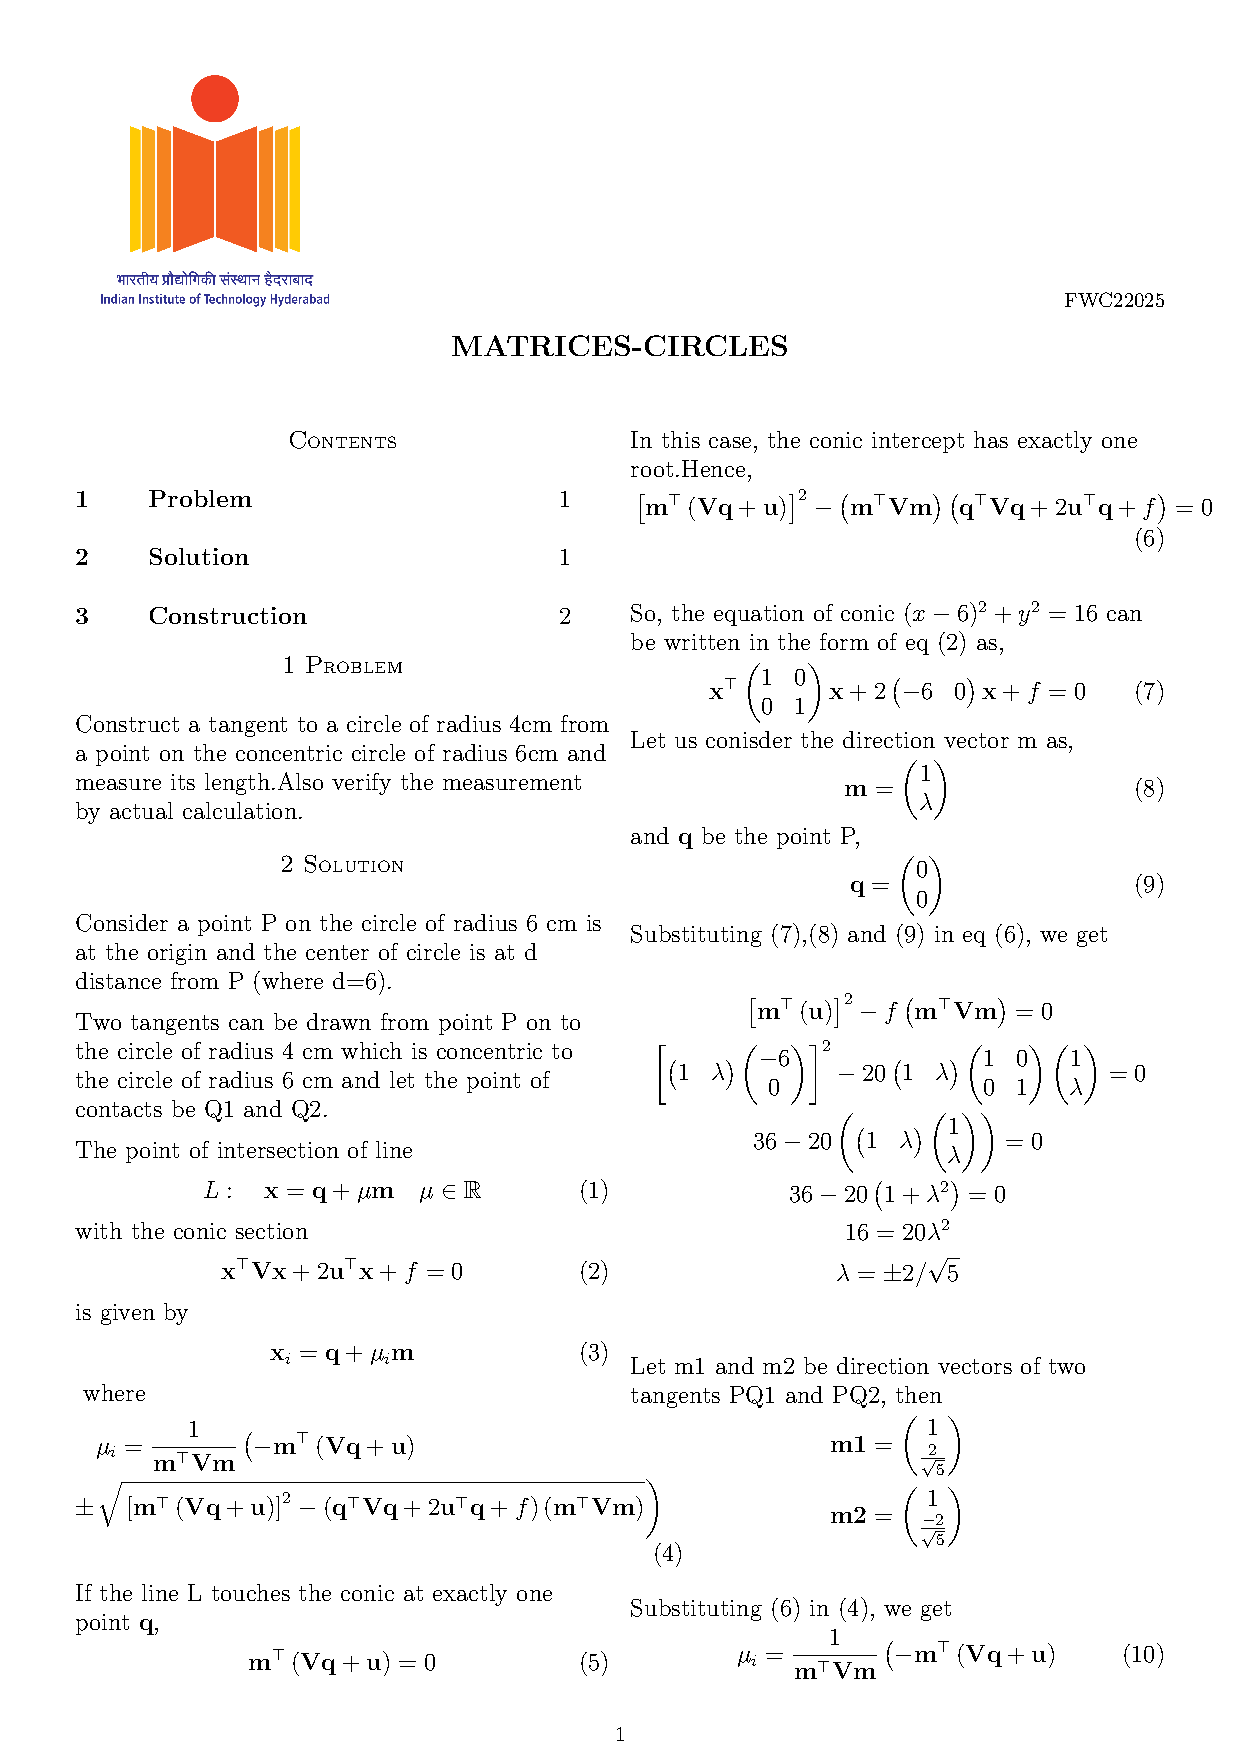
\includegraphics[scale=0.5]{fig/cir.pdf} \\
\caption{a circle passes through the point L and cuts the circle {$x^2+y^2=k^2$} orthogonally}
\end{figure}

\vspace{0.25cm}
With the given circle equation {$x^2+y^2=k^2$}, we can find out centre \(U_1\) and radius \(r_1\) of Circle-1
\vspace{0.25cm}
\textbf{STEP-1}

Centre of Circle-1,
\boldmath 
\begin{align} 
\vec{U_1} &= \begin{pmatrix}0 \\ 0 \\ \end{pmatrix} 
\end{align}
\unboldmath

Radius of Circle-1,
\boldmath
\begin{align}
 r_1  &= k
\end{align}
\unboldmath

\textbf{STEP-2}

let,the center of the  circle which passes through the point  L and cuts the circle {$x^2+y^2=k^2$} orthogonally is:
\boldmath 
\begin{align} 
\vec{U_2} = \begin{pmatrix}x \\ y \\ \end{pmatrix}
\end{align} 
\begin{align} 
\vec{L}= \begin{pmatrix}a \\ b \\ \end{pmatrix} 
\end{align}
\unboldmath
Radius of Circle be $r_2$

As both the circles are orthogonal, we get:\vspace{1mm}
\boldmath
\begin{align}
  ||\vec{U_2-U_1}||^2 &= r_1^2 +r_2^2
\end{align}


where

\begin{align}
\implies||\vec{U_2-U_1}||^2=||\vec{U_2}||^2 + ||\vec{U_1}||^2 - 2{\vec{U_1}}^{\top}\vec{U_2}
\end{align}

\begin{align}
\hspace{-3.25cm}\implies r_1^2=k^2\hspace{3cm}
\end{align}
$\implies r_2^2=||\vec{U_2-L}||^2$
\begin{align}
\hspace{-1.50cm}=||\vec{U_2}||^2+||\vec{L}||^2-2{\vec{L}}^{\top}\vec{U_2}
\end{align}
substitute equation (6),(7),(8) in equation (5)
$\implies ||{\vec{{U_2} - {U_1}}}||^2 = r_1^2 + r_2^2$\vspace{3mm}
$\implies ||\vec{U_2}||^2+||\vec{U_1}||^2-2\vec{U_1}^{\top}\vec{U_2}=$
\vspace{3mm}
\hspace{3cm}
$k^2+||\vec{U_2}||^2+||\vec{L}||^2-2{\vec{L}}^{\top}\vec{U_2}$
\unboldmath

by solving the above equation we get,
\boldmath
$\implies 2\vec{L}^{\top}\vec{U_2}=k^2+||\vec{L}||^2$
\begin{align}
\hspace{-4.25cm}\implies 2\vec{L}^{\top}\vec{U_2}=k^2+\vec{L}^{\top}\vec{L}
\end{align}

\unboldmath 

equation (9) is the required equation,which is a line eqaution
\boldmath
${n}^{\top}X=c$
\unboldmath

\section*{Construction}
\centering
\vspace{0.2cm}
{
\setlength\extrarowheight{2pt}
\begin{tabular}{|c|c|c|}
	\hline
	\textbf{Symbol}&\textbf{Value}&\textbf{Description}\\
	\hline
	$U_1$ & $\begin{pmatrix}0 \\ 0 \\ \end{pmatrix}$ & center of given circle\\
	\hline
	$r_1$ & k & radius of given circle\\
	\hline
	$U_2$ & $\begin{pmatrix}x \\ y \\ \end{pmatrix}$ & center of circle 2\\
	\hline
	$L$ & $\begin{pmatrix}a \\ b \\ \end{pmatrix}$ & a point on  circle 2\\
	\hline
	$r_2$ & $||{\vec{U_2}-\vec{L}}||^2$ & radius of circle 2\\
	\hline
\end{tabular}
}

\vspace{3cm}
Get the python code of the figures from
\begin{table}[h]
\large
\centering
\framebox{
\url{https://github.com/kkousar/KOUSAR_FWC/blob/main/circle_assignment/code/circle.py}}
\bibliographystyle{ieeetr}
\end{table}

\end{document}